% Composed-workflow figure for Ch20 ("Composing Tools & Orchestration") — the Vol 2 capstone.
% Standalone TikZ; compiled by `book-scaffold build-figures` via pdflatex -> pdftocairo -> SVG.
% Capability axis first (build-vs-buy -> subtract tools -> MCP -> shape I/O), then the coordination
% gate (work fans out? -> sub-agent/multi-agent with the ~15x cost gate, else stay single-agent).
% Every step debits one finite context window.
\documentclass[tikz,border=4mm]{standalone}
\usepackage{tikz}
\usetikzlibrary{positioning, arrows.meta, calc}

\begin{document}
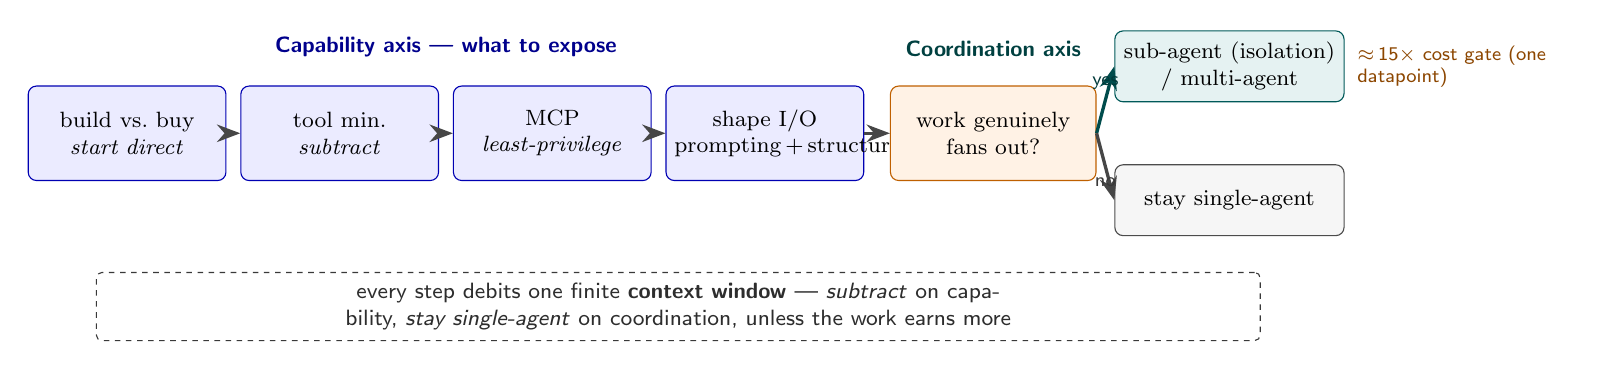
\begin{tikzpicture}[
  font=\sffamily,
  capbox/.style={draw=blue!70!black, fill=blue!8, rounded corners=3pt, align=center,
    text width=2.3cm, minimum height=1.2cm, inner sep=3pt, font=\footnotesize},
  gate/.style={draw=orange!75!black, fill=orange!10, rounded corners=3pt, align=center,
    text width=2.4cm, minimum height=1.2cm, inner sep=3pt, font=\footnotesize},
  outcome/.style={draw=teal!70!black, fill=teal!10, rounded corners=3pt, align=center,
    text width=2.7cm, minimum height=0.9cm, inner sep=3pt, font=\footnotesize},
  stay/.style={draw=gray!60!black, fill=gray!7, rounded corners=3pt, align=center,
    text width=2.7cm, minimum height=0.9cm, inner sep=3pt, font=\footnotesize},
  flow/.style={-Stealth, very thick, draw=gray!55!black}
]

% capability axis (left to right)
\node[capbox] (c1) at (0,0)    {build vs.\ buy\\\emph{start direct}};
\node[capbox] (c2) at (2.7,0)  {tool min.\\\emph{subtract}};
\node[capbox] (c3) at (5.4,0)  {MCP\\\emph{least-privilege}};
\node[capbox] (c4) at (8.1,0)  {shape I/O\\prompting\,+\,structured};
\node[font=\sffamily\bfseries\footnotesize, text=blue!55!black, anchor=south] at (4.05,0.85) {Capability axis — what to expose};

\draw[flow] (c1) -- (c2);
\draw[flow] (c2) -- (c3);
\draw[flow] (c3) -- (c4);

% coordination gate
\node[gate] (g) at (11.0,0) {work genuinely\\fans out?};
\draw[flow] (c4) -- (g);
\node[font=\sffamily\bfseries\footnotesize, text=teal!50!black, anchor=south] at (11.0,0.85) {Coordination axis};

\node[outcome] (yes) at (14.0,0.85) {sub-agent (isolation)\\/ multi-agent};
\node[stay] (no) at (14.0,-0.85) {stay single-agent};
\draw[flow, draw=teal!60!black] (g.east) -- (yes.west) node[midway, above=0pt, font=\sffamily\scriptsize, text=teal!45!black] {yes};
\draw[flow, draw=gray!55!black] (g.east) -- (no.west) node[midway, below=0pt, font=\sffamily\scriptsize, text=gray!45!black] {no};
\node[font=\sffamily\scriptsize, text=orange!55!black, anchor=west, text width=2.9cm] at (15.5,0.85) {$\approx$\,15$\times$ cost gate (one datapoint)};

% the banner
\node[draw=gray!45!black, dash pattern=on 2pt off 2pt, rounded corners=2pt, align=center,
  text width=14.5cm, inner sep=4pt, font=\sffamily\footnotesize, text=gray!35!black]
  at (7.0,-2.2) {every step debits one finite \textbf{context window} — \emph{subtract} on capability, \emph{stay single-agent} on coordination, unless the work earns more};

\end{tikzpicture}
\end{document}
